\documentclass[12pt]{article}
\usepackage{graphicx}
\usepackage[margin=30mm, paper = a4paper]{geometry}
\usepackage{minted, caption}
\usepackage{subcaption}
\usepackage{multicol}

\title{}
\author{}
\date{}
\setlength{\columnseprule}{1pt}
\setlength{\columnsep}{2cm}
\begin{document}
\vspace*{\fill}
\begin{center}

    \emph{Heaven's Light is Our Guide} \\
    \textbf{Rajshahi University of Engineering and Technology} \\

    \begin{figure}[h]
        \centering
        
\includegraphics[scale=.34]{images/RUET_logo.png}
        \label{fig:ruet_logo}
    \end{figure}
    \vspace{5mm}

    \textbf{Course Code}\\
    ECE 2216\\
    \vspace{3mm}
    \textbf{Course Title}\\
    Database Systems Sessional

    \vspace{5mm}
    \textbf{Experiment Date:} October 15, 2023,\\
    \textbf{Submission Date:} November 5, 2023\\

    \vspace{5mm}
    \textbf{Lab Report 3:} Creating a database and doing operations on it using SQL\\

    \vspace{15mm}

    \begin{tabular}{c|c}
        \textbf{Submitted to} & \textbf{Submitted by} \\
        Md. Robiul Islam      & Md. Tajim An Noor     \\
        Assistant Professor   & Roll: 2010025         \\
        Dept of ECE, Ruet     &                       \\
    \end{tabular}

\end{center}
\vspace*{\fill}

\pagebreak

\tableofcontents

\maketitle

\section{Tools Used}
\begin{itemize}
    \item MySQL
    \item VS Code - as an IDE to use SQL
    \item MacTeX -\LaTeX  compiler
    \item VS Code with LaTeX workshop extension as a text editor
\end{itemize}


\section{Process}
Create three tables in a database with primary and foreign keys and do operations on them.

\subsection*{SQL Codes:}

\subsubsection*{Creating tables and inserting data.}
\subsubsection*{Code:}
\begin{multicols}{2}{|}
    \begin{minted}[linenos,breaklines,breakanywhere]{mysql}
CREATE DATABASE IF NOT EXISTS Relations;
-- creating database and tables.
CREATE TABLE Relations.salesman(
    salesman_id int Auto_Increment Primary key,
    name VARCHAR(30),
    city VARCHAR(20),
    commission DECIMAL(4, 2)
);
--
CREATE TABLE Customer(
    customer_id int Auto_Increment Primary Key,
    customer_name varchar(40),
    city varchar(40),
    grade int,
    salesman_id int,
    Constraint cust_sales Foreign key (salesman_id) References salesman(salesman_id)
)
-- 
CREATE TABLE Relations.Order(
    order_no int Auto_Increment Primary Key,
    purchase_amount DECIMAL(6, 2),
    order_date Date,
    customer_id int,
    salesman_id int,
    Constraint cust_order Foreign key (customer_id) References Customer(customer_id),
    Constraint sales_order Foreign key (salesman_id) References salesman(salesman_id)
);
--
INSERT INTO
    Relations.salesman (salesman_id, name, city, commission)
VALUES
    (
        5001,
        'James Hoog',
        'New York',
        0.15
    ),
    (
        5002,
        'Nail Knite',
        'Paris',
        0.13
    ),
    (
        5003,
        'Lauson Hen',
        null,
        0.12
    ),
    (
        5005,
        'Pit Alex',
        'London',
        0.11
    ),
    (
        5006,
        'Mc Lyon',
        'New York',
        0.14
    ),
    (
        5007,
        'Pal Adam',
        'Rome',
        0.13
    );
--
INSERT INTO
    Relations.Customer (
        customer_id,
        customer_name,
        city,
        grade,
        salesman_id
    )
VALUES
    (
        3001,
        'Brad Guzan',
        'London',
        null,
        null
    ),
    (
        3002,
        'Nick Romando',
        'New York',
        100,
        5001
    ),
    (
        3003,
        'Jozy Altidor',
        'Moscow',
        200,
        5007
    ),
    (
        3004,
        'Fabian Johnson',
        'Paris',
        300,
        5006
    ),
    (
        3005,
        'Graham Zusi',
        'California',
        200,
        5002
    ),
    (
        3007,
        'Brad Davis',
        'New York',
        200,
        5001
    ),
    (
        3008,
        'Julian Green',
        'London',
        300,
        5002
    ),
    (
        3009,
        'Geoff Cameron',
        'Berlin',
        100,
        null
    );
--
INSERT INTO
    Relations.Order (
        order_no,
        purchase_amount,
        order_date,
        customer_id,
        salesman_id
    )
VALUES
    (
        70001,
        150.5,
        '2012-10-05',
        3005,
        5002
    ),
    (70002, 65.26, '2016-10-05', 3002, 5001),
    (70003, 2480.4, '2012-10-10', 3009, 5003),
    (70004, 110.5, '2012-08-17', 3009, 5003),
    (70005, 2400.6, '2012-07-27', 3007, 5001),
    (70007, 948.5, '2012-09-10', 3005, 5002),
    (70008, 5760, '2012-09-10', 3002, 5001),
    (70009, 270.65, '2012-09-10', 3001, 5005),
    (70010, 1983.43, '2012-10-10', 3004, 5006),
    (70011, 75.29, '2012-08-17', 3003, 5007),
    (70012, 250.45, '2012-06-27', 3008, 5002),
    (70013, 3045.6, '2012-04-25', 3002, 5001);
    \end{minted}
\end{multicols}

\vspace{10mm}


\subsubsection{Find the customer name who are given highest commission.}
\subsubsection*{Code:}
\begin{minted}[breaklines, linenos]{mysql}
SELECT
    customer_name as "Customer with highest Commission"
FROM
    Relations.Customer
WHERE
    Customer.customer_id = (
        SELECT
            Order.customer_id
        FROM
            Relations.Order
        ORDER BY
            Order.purchase_amount * (
                SELECT
                    salesman.commission
                FROM
                    Relations.salesman
                WHERE
                    salesman_id = Order.salesman_id
            ) DESC
        LIMIT
            1
    );
\end{minted}
\vspace{10mm}

\subsubsection{Find the amount of total commission given by salesman\_id = "5001".}
\subsubsection*{Code: }
\begin{minted}[breaklines, linenos]{mysql}
SELECT
    SUM(
        purchase_amount * (
            SELECT
                commission
            FROM
                Relations.salesman
            WHERE
                salesman_id = Order.salesman_id
        )
    ) AS "Total Commission",
    salesman_id as "Salesman ID"
FROM
    Relations.Order
WHERE
    Order.salesman_id = 5001;
\end{minted}

\vspace{10mm}

\subsubsection{Find the salesman name whose customer’s grade is lowest.}
\subsubsection*{Code: }
\begin{minted}[breaklines, breakanywhere, linenos]{mysql}
SELECT
    name as "Salesman Name"
FROM
    Relations.salesman
WHERE
    salesman_id IN (
        SELECT
            salesman_id
        FROM
            Relations.Customer
        WHERE
            grade IN (
                SELECT
                    MIN(grade)
                FROM
                    Relations.Customer
            )
    ) 
\end{minted}
\vspace{10mm}

\subsubsection{Find the total order number,ner from 5-9-2016 to 17-10-216 from the given table.}
\subsubsection*{Code: }
\begin{minted}[breaklines, breakanywhere, linenos]{mysql}
SELECT
    COUNT(order_no) as "Total order from 2016/9/5 to 2016/10/17"
FROM
    Relations.Order
WHERE
    order_date BETWEEN '2016-09-05'
    AND '2016-10-17';
\end{minted}


\section{Output}
\captionsetup{justification=centering}
\begin{figure}[htbp!]
    \begin{subfigure}{1\textwidth}
        \centering
        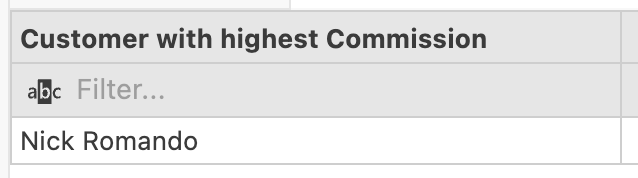
\includegraphics[width=\linewidth]{images/output/q1.png}
        \caption*{The person who is the top of the organization (i.e. reports to no one)}
        \label{fig:q1}
    \end{subfigure}
    \vspace*{20mm}
    \begin{subfigure}{.3\textwidth}
        \centering
        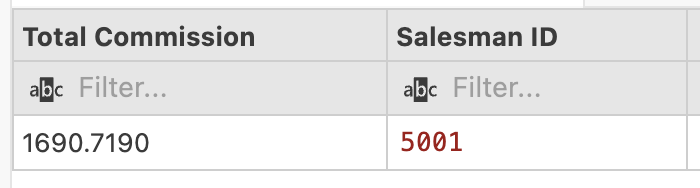
\includegraphics[width=.6\linewidth]{images/output/q2.png}
        \caption*{Difference in days between the most recent and oldest order date in Orders file.}
        \label{fig:q2}
    \end{subfigure}
    \begin{subfigure}{.3\textwidth}
        \centering
        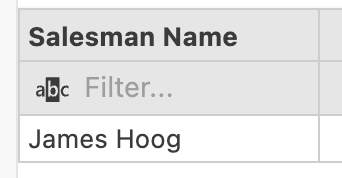
\includegraphics[width=.6\linewidth]{images/output/q3.png}
        \caption*{Total value of  payments received in July 2004.}
        \label{fig:q3}
    \end{subfigure}
    \begin{subfigure}{.3\textwidth}
        \centering
        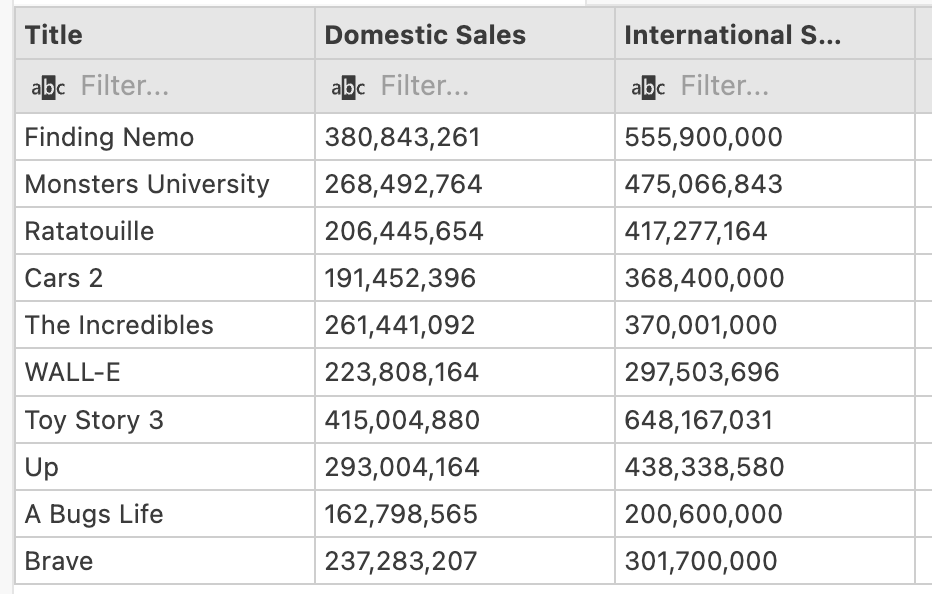
\includegraphics[width=.6\linewidth]{images/output/q6.png}
        \caption*{The number of orders ‘On Hold’ for each customer.}
        \label{fig:q6}
    \end{subfigure}

    \begin{subfigure}{\textwidth}
        \centering
        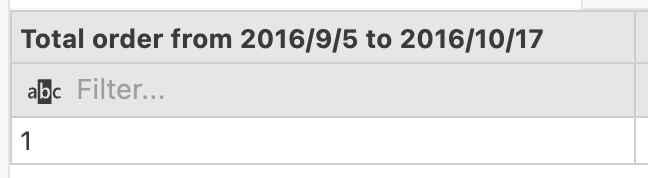
\includegraphics[width=.5\linewidth]{images/output/q4.png}
        \caption*{Profit generated by each sales representative based on the orders from the customers they serve. Sorted by profit generated descending.}
        \label{fig:q4}
    \end{subfigure}
    \begin{subfigure}{.5\textwidth}
        \centering
        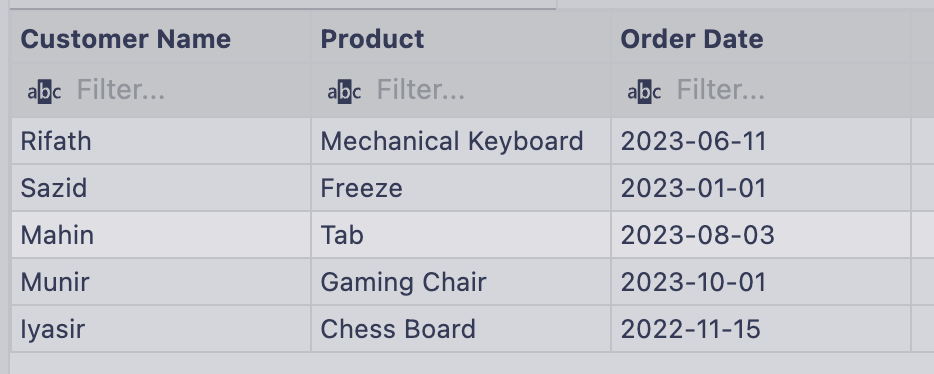
\includegraphics[width=.8\linewidth]{images/output/q5.png}
        \caption*{Products sold in 2003 but not 2004.}
        \label{fig:q5}
    \end{subfigure}
    \begin{subfigure}{.5\textwidth}
        \centering
        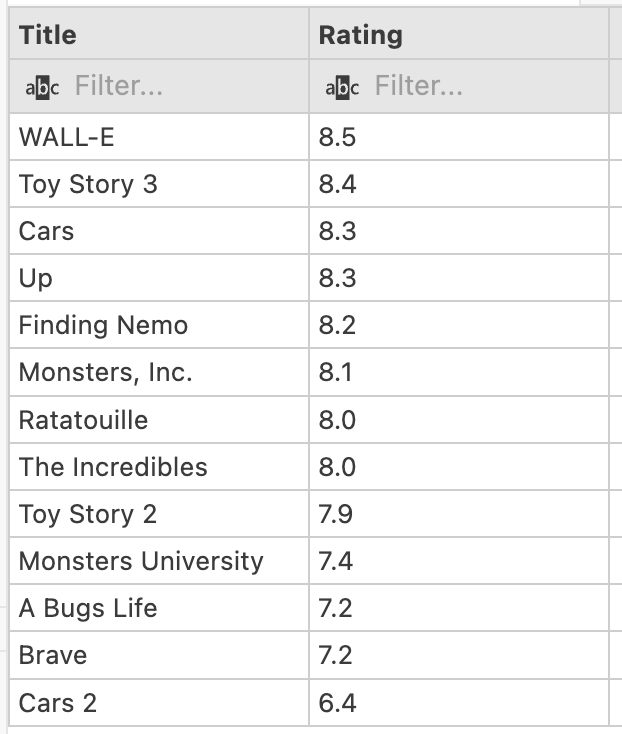
\includegraphics[width=.65\linewidth]{images/output/q7.png}
        \caption*{Names of products sold at less than 80\% of the MSRP.}
        \label{fig:q7}
    \end{subfigure}
\end{figure}


\end{document}